\def\duedate{\today}
\def\HWnum{1}
\documentclass[10pt,a4paper]{book}

% custom section formatting
\usepackage{titlesec}
\titleformat{\chapter}[display]
{\normalfont\Large\filcenter\sffamily}
{\titlerule[1pt]%
\vspace{1pt}%
\titlerule
\vspace{1pc}%
\LARGE\MakeUppercase{\chaptertitlename} \thechapter}
{1pc}
{\titlerule
\vspace{1pc}%
\Huge}

% appendix handling
\usepackage[toc,page]{appendix}
    
% encoding for file and font
\usepackage[utf8]{inputenc}
\usepackage[T1]{fontenc}

% math formatting/tools
\usepackage{amsmath}
\usepackage{amssymb}
\usepackage{mathtools}
\usepackage[arrowdel]{physics}

% unit formatting
\usepackage{siunitx}
\AtBeginDocument{\RenewCommandCopy\qty\SI}

% figure formatting/tools
\usepackage{graphicx}
\usepackage{float}
\usepackage{subcaption}
\usepackage{multirow}
\usepackage{import}
\usepackage{pdfpages}
\usepackage{transparent}
\usepackage{currfile}

\NewDocumentCommand\incfig{O{1} m}{
    \def\svgwidth{#1\textwidth}
    \import{./Figures/\currfiledir}{#2.pdf_tex}
}

\newcommand{\bef}{\begin{figure}[h!tb]\centering}
\newcommand{\eef}{\end{figure}}

\newcommand{\bet}{\begin{table}[h!tb]\centering}
\newcommand{\eet}{\end{table}}

% hyperlink references 
\usepackage{hyperref}
\hypersetup{
    colorlinks=true,
    linkcolor=blue,
    filecolor=magenta,
    urlcolor=cyan,
    pdftitle={Physics 1 Notes},
    pdfauthor={Richard Whitehill},
    pdfpagemode=FullScreen
}
\urlstyle{same}

\newcommand{\eref}[1]{Eq.~(\ref{eq:#1})}
\newcommand{\erefs}[2]{Eqs.~(\ref{eq:#1})--(\ref{eq:#2})}

\newcommand{\fref}[1]{Fig.~(\ref{fig:#1})}
\newcommand{\frefs}[2]{Fig.~(\ref{fig:#1})--(\ref{fig:#2})}

\newcommand{\aref}[1]{Appendix~(\ref{app:#1})}
\newcommand{\sref}[1]{Section~(\ref{sec:#1})}
\newcommand{\srefs}[2]{Sections~(\ref{sec:#1})-(\ref{sec:#2})}

\newcommand{\tref}[1]{Table~(\ref{tab:#1})}
\newcommand{\trefs}[2]{Table~(\ref{tab:#1})--(\ref{tab:#2})}

% tcolorbox formatting/definitions
\usepackage[most]{tcolorbox}
\usepackage{xcolor}
\usepackage{xifthen}
\usepackage{parskip}

\definecolor{peach}{rgb}{1.0,0.8,0.64}

\DeclareTColorBox[auto counter, number within=chapter]{defbox}{O{}}{
    enhanced,
    boxrule=0pt,
    frame hidden,
    borderline west={4pt}{0pt}{green!50!black},
    colback=green!5,
    before upper=\textbf{Definition \thetcbcounter \ifthenelse{\isempty{#1}}{}{: #1} \\ },
    sharp corners
}

\newcommand*{\eqbox}{\tcboxmath[
    enhanced,
    colback=black!10!white,
    colframe=black,
    sharp corners,
    size=fbox,
    boxsep=8pt,
    boxrule=1pt
]}

\newtcolorbox[auto counter, number within=chapter]{exbox}{
    parbox=false,
    breakable,
    enhanced,
    sharp corners,
    boxrule=1pt,
    colback=white,
    colframe=black,
    before upper= \textbf{Example \thetcbcounter:}\,,
    before lower= \textbf{Solution:}\,,
    segmentation hidden
}

\newtcolorbox{resbox}{
    enhanced,
    colback=black!10!white,
    colframe=black,
    boxrule=1pt,
    boxsep=0pt,
    top=2pt,
    ams nodisplayskip,
    sharp corners
}


\begin{document}


\prob{1 -- Ch. 1 \#3}{

Consider the Rutherford model of the atom: an electron of electric charge $-e$ orbiting a point-like nucleus (much heavier, and hence at rest) of electric charge $Ze$ in a circular orbit of radius $R$.
Knowing that the electron radiates energy away at the rate $\dd{E}/\dd{t}$ given by 
\begin{eqnarray}
    \dv{E}{t} = -\frac{2}{3} \frac{e^2 |\va*{a}(t)|^2}{c^3}
,\end{eqnarray}
where $\va*{a}(t)$ is the acceleration and $c$ is the speed of light, show that it will take a time
\begin{eqnarray}
   \tau = \frac{m^2 c^3}{Z e^{4}} \frac{R^3}{4}
\end{eqnarray}
for the electron to spiral into the nucleus.
Assume that $\tau$ is much larger than the revolution period.
By taking $Z=1$ and $R \approx \SI{1e-8}{\centi\metre}$ appropriate for the hydrogen atom, justify this assumption \textit{a posteriori} by comparing $\tau$ with the revolution period.


}

\sol{

The energy of this system is
\begin{eqnarray}
   E = \frac{1}{2} m v^2 - \frac{Z e^2}{r}
,\end{eqnarray}
when the electron is at a distance $r$ from the nucleus.
Since the acceleration is instantaneously centripetal\footnote{This is approximately true if we assume that the energy lost per revolution is much smaller than the energy of the system, and thus, that the electron's tangential component of acceleration is very small.} we can write
\begin{eqnarray}
    ma = m\frac{v^2}{r} = \frac{Ze^2}{r^2} \Rightarrow T = \frac{1}{2} V
.\end{eqnarray}
Actually, this is a version of the Virial Theorem for inverse square power laws.
Using this, we find
\begin{eqnarray}
   E = -\frac{1}{2} \frac{Z e^2}{r}
.\end{eqnarray}
From here, we can differentiate this expression of $E$ giving
\begin{eqnarray}
    \dv{E}{t} = \frac{1}{2} \frac{Ze^2}{r^2} \dv{r}{t} = -\frac{2 e^2}{3 c^3} \frac{1}{m^2} \Big( \frac{Ze^2}{r^2} \Big)^2
.\end{eqnarray}
Solving for $\dd{r}/\dd{t}$ gives
\begin{eqnarray}
    \dv{r}{t} = -\frac{4 e^2}{3c^3} \frac{1}{m^2} \frac{Z e ^2}{r^2}
.\end{eqnarray}
We can solve this differential equation as follows
\begin{eqnarray}
    \int_{r(0)}^{r(\tau)} r^{2} \dd{r} = -\frac{R^3}{3} = -\frac{4 Z e^{4}}{3 m^2 c^3} \tau
.\end{eqnarray}
And finally we rearrange to find 
\begin{eqnarray}
    \eqbox{ \tau = \frac{m^2 c^3}{Z e^{4}} \frac{R^3}{4} \approx Z \times 10^{-10}~{\rm s}}
,\end{eqnarray}
for the conditions stated above.

Note that a distance $R$ from the center one orbital period is
\begin{eqnarray}
    T = 2 \pi \sqrt{ \frac{R^3 m}{Z e ^2}} \approx \frac{1}{\sqrt{Z}} (4 \times 10^{-16}~{\rm s})
,\end{eqnarray}
and hence, the proportion of one period to the time of the electron's orbital decay is given as
\begin{eqnarray}
    \frac{T}{\tau} \approx 4\sqrt{Z} \times 10^{-6}
,\end{eqnarray}
which is quite tiny for any relevant $Z$ and at least tells us that our results are consistent with our assumptions.


}


\prob{2 -- Ch. 1 \#7}{

In addition to its failures in explaining the blackbody radiation spectrum, the photo-electric effect, and the stability of atoms and spectral lines, classical physics could also not explain the heat capacity of a solid. \\[3pt]

(a) Assume a solid of volume $V$ with $N$ atoms (or molecules) can be modeled as a set of $3N$ independent one-dimensional harmonic oscillators of frequency $\nu_0$ (that is, all oscillators have the same frequency $\nu_0$).
Making use of the equipartition theorem, calculate the total average energy $E$ of the solid at temperature $T$ and derive the Dulong-Petit law for the heat capacity (at constant volume)
\begin{eqnarray}
    c_{V} = \Big( \pdv{E}{T} \Big)_{V} = 3 N k_{B}
,\end{eqnarray}
where $k_{B}$ is the Boltzmann's constant. \\[3pt]

(b) The observed heat capacity of a solid is not a constant independent of $T$, but rather vanishes as $T^3$ at low temperature and approaches the classical prediction (the Dulong-Petit law) at high temperature.
Einstein (1907) proposed that the energy of each harmonic oscillator is quantized and that its average energy at temperature $T$ is given by
\begin{eqnarray}
    \expval{E} = \frac{h \nu_0}{\exp(h \nu_0/k_{B}T) - 1}
,\end{eqnarray}
see class notes.
Show that the heat capacity is now found to be
\begin{eqnarray}
    c_{V} = 3 N k_{B} \frac{x_0^2 e^{x_0}}{(e^{x_0}-1)^2}, \quad x_0 = \frac{h \nu_0}{k_{B} T}
.\end{eqnarray}
Does $c_{V}$ vanish as $T \rightarrow 0$?
What happens at high temperature? \\[3pt]

(c) Einstein's theory predicts that $c_{V}$ vanishes exponentially at low temperature, a result that is at variance with experimental observations.
A more realistic model of a solid is that it consists of $3N$ independent harmonic oscillators (modes) with a distribution in frequency $g(\nu)$ given by
\begin{eqnarray}
    g(\nu) = 4\pi \frac{V}{v_{S}^3} \nu^2
,\end{eqnarray}
where $v_{S}$ is the sound velocity in the solid, such that 
\begin{eqnarray}
    {\rm number~of~modes} = \int_{0}^{\nu_{\rm max}} \dd{\nu} g(\nu) = 3N
.\end{eqnarray}
This condition fixes $\nu_{\rm max}$ as a function of the density $N/V$.
Introduce the parameter $T_{D}$ (the Debye temperature) defined as $T_{D} = h \nu_{\rm max}/k_{B}$ and show that the total average energy at temperature $T$ is given by
\begin{eqnarray}
    E = 9 N h \nu_{\rm max} \Big( \frac{T}{T_{D}} \Big)^{4} \int_{0}^{T_{D}/T} \dd{x} \frac{x^3}{e^{x} - 1}
,\end{eqnarray}
and that the constant-volume heat capacity is proportional to $T^3$ for low $T$, in agreement with experiment.
Show that it also satisfies the Dulong-Petit law at high temperatures.

}


\sol{

(a) The Hamiltonian for a 1D harmonic oscillator is given by
\begin{eqnarray}
   H = \frac{p^2}{2m} + \frac{m \omega_0^2}{2} q^2 
,\end{eqnarray}
where $p$ and $q$ are the generalized momentum and spatial variables of the oscillator and $\omega_0 = 2 \pi \nu_{0}$ is the angular frequency of the oscillator.
The equipartition theorem states that for a system
\begin{eqnarray}
   E = \sum_{\rm particles} \sum_{\rm d.o.f.} \frac{1}{2} k_{B} T = 3 N k_{B} T
.\end{eqnarray}
From this, the heat capacity of a solid modeled in this way is
\begin{eqnarray}
    \eqbox{ c_{V} = \Big( \pdv{E}{T} \Big)_{V} = 3 N k_{B} }
,\end{eqnarray}
which is constant with temperature.

(b) We can derive the average energy for an oscillator at temperature $T$ using some basic results from statistical mechanics.
Namely, the energy of an ensemble is given by
\begin{eqnarray}
    \expval{E} = -\frac{1}{\cal Z} \pdv{Z}{\beta} = -\pdv{\ln{\cal Z}}{\beta}
,\end{eqnarray}
where $\cal Z$ is the partition function of our ensemble and defined as
\begin{eqnarray}
    {\cal Z} = \sum_{i} e^{-\beta E_{i}}
,\end{eqnarray}
where $\beta^{-1} = k_{B}T$.
In our case, the energy of an oscillator with frequency $\nu_0$ is quantized (per Einstein's postulate) as $E_{n} = n h \nu_0$.
Putting this into the partition function definition, we find
\begin{eqnarray}
    {\cal Z} = \sum_{n} (e^{- \beta h \nu_0})^{n} = \frac{1}{1 - e^{-\beta h \nu_0}}
.\end{eqnarray}
Hence, the average energy of an oscillator is 
\begin{eqnarray}
    \begin{aligned}
        \expval{E} &= - (1 - e^{-\beta h \nu_0}) \pdv{\beta} \Big[ \frac{1}{1 - e^{-\beta h \nu_0}} \Big] \\
                   &= -(1 - e^{-\beta h \nu_0}) [-(1 - e^{-\beta h \nu_0})^{-2} (h \nu_0) e^{-\beta h \nu_0}] \\
                   &= \frac{h \nu_0}{e^{\beta h \nu_0} - 1}
    \end{aligned}
,\end{eqnarray}
which is the result quoted above.

Now, we can derive the heat capacity of a solid by setting the energy of the solid to be $E = 3 N \expval{E_{\rm o}}$.
Then
\begin{eqnarray}
    \begin{aligned}
        c_{V} &= 3N \Big( \pdv{\expval{E}}{T} \Big)_{V} = 3N \Big( -\frac{\beta^2}{k_{B}} \Big) \pdv{\expval{E}}{\beta} \\
              &= \frac{3 N \beta^2}{k_{B}} \frac{(h \nu_0)^2 e^{\beta h \nu_0}}{(e^{\beta h \nu_0} - 1)^2}
    .\end{aligned}
\end{eqnarray}
If we rewrite our result in terms of the dimensionless variable $x_0 = \beta h \nu_0$, we have
\begin{eqnarray}
    \eqbox{ c_{V} = \frac{3N}{k_{B}} \frac{x_0^2 e^{x_0}}{(e^{x_0} - 1)^2} }
.\end{eqnarray}
From this expression, we can evaluate the extreme behavior of this function.
First, as $T \rightarrow 0$, $x_0 \rightarrow \infty$ and $c_{V} \rightarrow 0$ since the term $e^{2x_0}$ in the denominator dominates the expression at large $x_0$, meaning that $c_{V}$ vanishes exponentially fast at small temperatures.
Additionally, for large temperatures $T$ (and thus $x_0 \approx 0$), we find
\begin{eqnarray}
    c_{V} = 1 - \frac{x_0^2}{12} + {\cal O}(x_0^{4}) \rightarrow 1 ~{\rm as}~ T \rightarrow \infty
.\end{eqnarray}

(c) To correct Einstein's prediction, we allow the modes to oscillate at independent frequencies $\nu \in [0,\nu_{\rm max}]$ with a distribution $g(\nu) = 4 \pi (V/v_{S}^3) \nu^2$.
We can solve for $\nu_{\rm max}$ as follows:
\begin{eqnarray}
    4 \pi \frac{V}{v_{S}^3} \int_{0}^{\nu_{\rm max}} \dd{\nu} \nu^2 = \frac{4 \pi}{3} \frac{V}{v_{S}^3} \nu_{\rm max}^3 = 3 N \Rightarrow \nu_{\rm max} = \Big[ \frac{9}{4 \pi} \Big( \frac{N}{V} \Big) \Big]^{1/3} v_{S}
.\end{eqnarray}
At this point, the average energy of the solid is given simply as 
\begin{eqnarray}
    E = \int_{0}^{\nu_{\rm max}} g(\nu) \frac{h \nu}{e^{\beta h \nu} - 1} \dd{\nu}
.\end{eqnarray}
Switching to a dimensionless integration variable $x = \beta h \nu$ we find
\begin{eqnarray}
    \begin{aligned}
        E &= \frac{9 N}{\nu_{\rm max}^3} \int_{0}^{T_{D}/T} \Big( \frac{x}{\beta h} \Big)^2 \frac{1}{\beta} \frac{x}{e^{x} - 1} \Big( \frac{1}{\beta h} \Big) \dd{x} \\
          &= \frac{9 N}{\nu_{\rm max}^3 \beta^{4} h^3} \int_{0}^{T_{D}/T} \frac{x^3}{e^{x}-1} \dd{x} \\
          &= 9 N h \nu_{\rm max} \Big( \frac{1}{\beta h \nu_{\rm max}} \Big)^{4} \int_{0}^{T_{D}/T} \frac{x^3}{e^{x} - 1} \dd{x} \\
          &= \eqbox{9 N h \nu_{\rm max} \Big( \frac{T}{T_{D}} \Big)^{4} \int_{0}^{T_{D}/T} \frac{x^3}{e^{x} - 1} \dd{x} }
    \end{aligned}
,\end{eqnarray}
where we have expressed $\nu_{\rm max}$ in terms of $T_{D}$ and $g(\nu) = 9 N \nu^2 / \nu_{\rm max}^3$.

Let us now evaluate the behavior of $c_{V}$ for extreme temperatures

Now, the heat capacity of the solid is given as
\begin{eqnarray}
    c_{V} = 9 N h \nu_{\rm max} \pdv{T} \Bigg[ \Big( \frac{T}{T_{D}} \Big)^{4} \int_{0}^{T_{D}/T}\frac{x^3}{e^{x} - 1} \dd{x} \Bigg]
.\end{eqnarray}
Note that the physics is contained in the derivative of the factor in brackets, so for our analysis we only consider this term, which we denote $\tilde{c}_{V}$.
Carrying out the arithmetic, we have 
\begin{eqnarray}
   \begin{aligned}
       \tilde{c}_{V} &= \frac{4}{T_{D}} \Big( \frac{T}{T_{D}} \Big)^{3} \int_{0}^{T_{D}/T} \frac{x^3}{e^{x} - 1} \dd{x} + \Big( \frac{T}{T_{D}} \Big)^{4} \Big( -\frac{T_{D}}{T^2} \Big) \frac{(T_{D}/T)^3}{e^{T_{D}/T} - 1} \\
                     &= T^3 \Bigg[ \frac{4}{T_{D}^{4}} \int_{0}^{T_{D}/T} \frac{x^{3}}{e^{x} - 1} \dd{x} - \frac{1}{T^{4}(e^{T_{D}/T} - 1)} \Bigg]
   \end{aligned} 
.\end{eqnarray}
If we consider $T \rightarrow 0$, then
\begin{eqnarray}
    \eqbox{ \tilde{c}_{V} \approx T^3 \Bigg[ \frac{4}{T_{D}^{4}} \int_{0}^{\infty} \frac{x^3}{e^{x} - 1} \dd{x} \Bigg] }
,\end{eqnarray}
which has the desired behavior.

At large temperatures (i.e. $T \rightarrow \infty$), we have
\begin{eqnarray}
    \begin{aligned}
        \tilde{c}_{V} &\approx \frac{4T^3}{T_{D}^{4}} \int_{0}^{T_{D}/T} [x^2 + {\cal O}(x^3)] \dd{x} - \frac{1}{T[ (1 + T_{D}/T + {\cal O}(T_{D}^2/T^2)) - 1 ]} \\
                      &\approx \frac{4}{3 T_{D}} - \frac{1}{T_{D}} = \frac{1}{3 T_{D}} = \frac{1}{3} \frac{k_{B}}{h \nu_{\rm max}}
    \end{aligned}
,\end{eqnarray}
and therefore
\begin{eqnarray}
    \eqbox{ c_{V} = 3 N k_{B} }
.\end{eqnarray}

\textit{ In retrospect, it is likely simpler to define $\tilde{E} = E/(9 N h \nu_{\rm max})$, consider the limiting behavior of $\tilde{E}(T)$, and let $\tilde{c}_{V} = (\partial_{T} \tilde{E})_{V}$.
From this approach, we only have to keep track of one term instead of two, which is certainly cleaner. }


}


\prob{3 -- Ch. 2 \# 2}{

A beam of neutrons having energy $E$ is incident on a linear chain of atomic nuclei.
The chain is oriented perpendicularly to the beam.
The nuclei are located along the chain at regular intervals separated by a distance $d$, which is much larger than the radius $R$ of the nucleus.
A neutron detector is positioned far away from the chain and in a direction making an angle $\theta$ with the direction of the incident beam.
The mass of the neutron is $M = 1.67 \times 10^{-24}~{\rm g}$. \\[3pt]

(a) Describe qualitatively the phenomenon observed at the detector as the energy $E$ of the incident neutrons is changed (\textbf{Hint}: think of Bragg's reflection and obtain the condition for its occurence). \\[3pt]

(b) The counting rate (or intensity), as a function of $E$, presents a resonance (peak) when $E = E_1$.
Knowing that there are no other resonances for $E < E_1$, show that the separation distance $d$ between contiguous nuclei can be determined.
Calculate $d$ when $\theta = 30^{\circ}$ and $E_1 = 1.3 \times 10^{-13}~{\rm erg}$. \\[3pt]

(c) At about what value of $E$ must we be taking the nuclear size into account.
Take $R \approx 10^{-13}~{\rm cm}$.

}

\begin{figure}[h!tb]
   \centering
   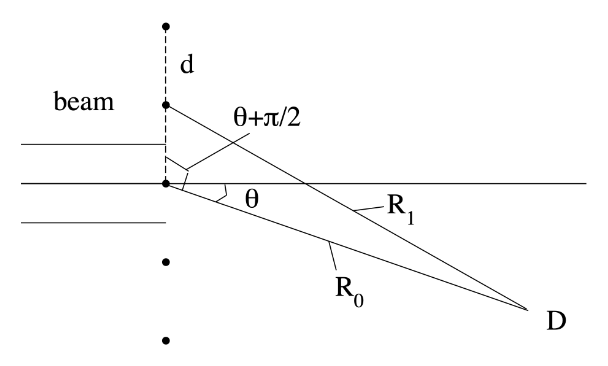
\includegraphics[width=0.5\textwidth]{prob3.png}
   \label{fig:prob3}
   \caption{A beam of neutrons incident on a linear chain of nuclei.}
\end{figure}

\sol{

(a)

(b)

(c) The ``rule of thumb'' for when the size of the target particle must be taken into acccount is when the wavelength of the incoming particles is on the same scale as the size of the target particles, which in this case is about $1~{\rm fm}$ or $10^{-13}~{\rm cm}$.
Doing the quick estimations, we find
\begin{eqnarray}
   \lambda_{N} = \frac{h}{p(E)} = \frac{h}{?}
.\end{eqnarray}
{\color{red} Are the neutrons relativistic at this scale?}

}


\prob{4 -- Ch. 2 \#5}{

Consider a wave packet in three dimensions
\begin{eqnarray}
    \Psi(\va*{r},t) = \int \frac{\dd^3{\va*{k}'}}{(2 \pi)^{3/2}} f(\va*{k}') e^{i(\va*{k}' \cdot \va*{r} - \omega' t)}
,\end{eqnarray}
and assume that the dependence of $\omega'$ on $\va*{k}'$ is not specified; in other words, assume that $\omega' = \omega'(\va*{k}')$. \\[3pt]

(a) Suppose $f(\va*{k}') \ne 0$ only for $\va*{k}'$ in a small region around $\va*{k}$.
By expanding $\omega'$ in Taylor series around $\va*{k}' = \va*{k}$ up to linear terms in $\va*{k}' - \va*{k}$, show that 
\begin{eqnarray}
    \Psi(\va*{r},t) \approx e^{-i(\omega - \va*{k} \cdot \grad_{\va*{k}}{\omega})t} \Psi(\va*{r} - \grad_{\va*{k}} \omega t, 0)
,\end{eqnarray}
where we have defined $\omega = \omega'(\va*{k})$ and $\grad_{\va*{k}} \omega = \grad_{\va*{k}'} \omega'|_{\va*{k}' = \va*{k}}$.
Consider the shape of the wave packet $|\Psi(\va*{r},t)|$.
What does the relation above imply about the change of this shape with time? \\[3pt]

(b) From the relation obtained in part (a) deduce that the wave packet travels with the velocity -- the so-called group velocity $\va*{v}_{\rm gr}$ -- given by $\grad_{\va*{k}} \omega$.
Identifying this velocity as the velocity $\hbar \va*{k}/m$ of the particle, where $m$ is its mass, show that 
\begin{eqnarray}
    \omega = \frac{\hbar k^2}{2m} + {\rm constant} 
.\end{eqnarray}


}

\sol{

If we assume that $|f(\va*{k}')|$ is strongly localized in a neighborhood of $\va*{k}' = \va*{k}$, we can linearize $\omega'$ as 
\begin{eqnarray}
   \omega' \approx \omega +  (\va*{k}' - \va*{k}) \cdot \grad_{\va*{k}'} \omega' |_{\va*{k}' = \va*{k}}
.\end{eqnarray}
In this case, we can then write $\Psi$ as
\begin{eqnarray}
    \Psi(\va*{r},t) \approx \int \frac{\dd[3]{\va*{k}'}}{(2\pi)^{3/2}} f(\va*{k}') e^{i \big( \va*{k}' \cdot \va*{r} - \big[ \omega + (\va*{k}' - \va*{k}) \cdot \grad_{\va*{k}'} \omega'|_{\va*{k}' = \va*{k}} \big] t \big)}
.\end{eqnarray}
We can then take out any exponential factor which are independent of $\va*{k}'$, which gives
\begin{eqnarray}
    \eqbox{
    \begin{aligned}
        \Psi(\va*{r},t) &\approx e^{-i \big( \omega - \va*{k} \cdot \grad_{\va*{k}'} \omega' |_{\va*{k}' = \va*{k}} \big) t} \int \frac{\dd[3]{\va*{k}'}}{(2\pi)^{3/2}} f(\va*{k}') e^{i \va*{k}' ( \va*{r} - t \grad_{\va*{k}'} \omega'|_{\va*{k}' = \va*{k}} )} \\
                        &= e^{-i \big( \omega - \va*{k} \cdot \grad_{\va*{k}'} \omega' |_{\va*{k}' = \va*{k}} \big) t} \Psi(\va*{r} - t \grad_{\va*{k}'} \omega'|_{\va*{k}'} = \va*{k}, 0)
    \end{aligned}
}
.\end{eqnarray}
Note that the factor $\grad_{\va*{k}'} \omega'|_{\va*{k}' = \va*{k}}$ is in fact independent of $\va*{k}'$ since we make the replacement $\va*{k}' = \va*{k}$ after taking the gradient with respect to $\va*{k}'$.

}



\end{document}
